\sloppy
\section{Environment Setup}
\begin{figure}[ht]
	\centerline{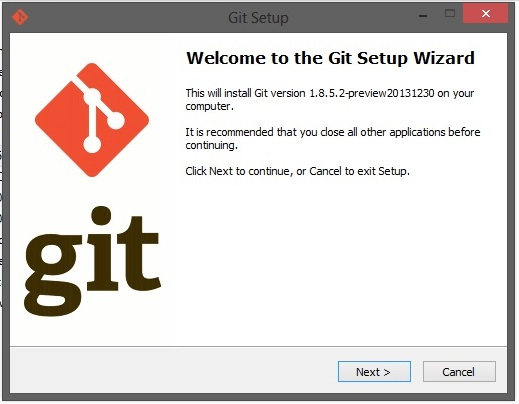
\includegraphics[width=0.25\textwidth]{Figures/gitenvirontment}}
	\caption{git setup environtment}
	\label{gitenvirontment}
\end{figure}
\vspace{12pt}
\noindent 
Tutorial ini menuntun Anda melalui cara menyiapkan Git di berbagai platform sehingga Anda bisa membaca dan menulis kode YUI dalam waktu singkat. $  $Setelah lingkungan Anda diatur, pastikan untuk membaca tutorial $  $untuk belajar bagaimana mengkloning kode sumber YUI ke lingkungan pengembangan lokal Anda, dan kiriman CLA untuk berkontribusi pada YUI. \par
\vspace{12pt}
\noindent
\begin{verbatim}
Instal Git di Mac
\end{verbatim} 
 
\vspace{12pt}
\noindent 
 $  $Singa \par
\vspace{12pt}
\noindent 
Download dan Install Xcode dari Mac App Store (gratis) \par
\noindent 
Setelah instalasi buka terminal dan ketik: $  $git --version \par
\noindent 
Anda harus melihat sesuatu seperti $  $Versi $  $ini $  $dapat bervariasi $  $: $  $git version 1.7.4.4 \par
\noindent 
Git sekarang terpasang dan bekerja \par
\vspace{12pt}
\noindent 
 $  $[Macan Tutul Salju \par
\vspace{12pt}
\noindent 
Download dan Instal Git Client untuk OS X  \par
\noindent 
Setelah instalasi buka terminal dan ketik: $  $git --version \par
\noindent 
Anda harus melihat sesuatu seperti $  $Versi $  $ini $  $dapat bervariasi $  $: $  $git version 1.7.6.1 \par
\noindent 
Git sekarang terpasang dan bekerja \par
\vspace{12pt}
\noindent 
 $  $Harimau \par
\vspace{12pt}
\noindent 
Download dan Install paket Git untuk OS X  \par
\noindent 
Anda perlu menambahkan $  $/usr/local/bin $  $ke $  $ $  \$  $PATH \par
\noindent 
vim  $  \sim  $/.bashrc \par
\vspace{12pt}
\noindent 
Di bagian bawah file tambahkan baris ini: \par
\noindent 
ekspor $  $PATH= $  \$  $PATH:/usr/local/bin \par
\vspace{12pt}
\noindent 
Setelah instalasi buka terminal dan ketik: $  $git --version \par
\noindent 
Anda harus melihat sesuatu seperti ini: $  $git version 1.7.6.1 \par
\noindent 
Git sekarang terpasang dan bekerja \par
\vspace{12pt}
\noindent 
\subsection{Port Mac}
\vspace{12pt}
\noindent 
Jika Anda menginstal Mac Ports, lakukan hal berikut: \par
\vspace{12pt}
\noindent
\begin{verbatim}
Instal paket
  $git-core
 

sudo port install git-core \par
Setelah instalasi buka terminal dan ketik: $  $git --version \par
Anda harus melihat sesuatu seperti ini: $  $git version 1.6.0 \par
 
Git sekarang terpasang dan bekerja \par

\end{verbatim} 
\noindent 
 $  $Pengadu \par
\vspace{12pt}
\noindent 
Git ada di pohon yang tidak stabil di Fink, dan aku tidak bisa memasangnya. $  $Anda harus memilih metode lain \par
\vspace{12pt}
\noindent 
 $  $Instal Git di Linux \par
\vspace{12pt}
\noindent 
 $  $Topi merah \par
\vspace{12pt}
\noindent 
Untuk Fedora 7 dan yang lebih baru. \par
\vspace{12pt}
\noindent 
Instal paket $  $git-core \par
\noindent 
sudo yum install git-core \par
\vspace{12pt}
\noindent 
Setelah instalasi buka terminal dan ketik: $  $git --version \par
\noindent 
Anda harus melihat sesuatu seperti ini: $  $git version 1.7.6.1 \par
\vspace{12pt}
\noindent 
Git sekarang terpasang dan bekerja \par
\vspace{12pt}
\noindent 
Untuk Fedora 6 dan yang lebih tua, git-core adalah bagian dari Fedora Extras  \par
\vspace{12pt}
\noindent 
Bagi pengguna Red Hat Enterprise Linux dan klonnya (seperti CentOS dan Scientific Linux), pengguna harus membangun git dengan tangan. $  $Sumber tersedia di sini: $  $http://git.or.cz/ \par
\vspace{12pt}
\noindent 
 $  $Ubuntu \par
\vspace{12pt}
\noindent 
Instal paket $  $git-core \par
\vspace{12pt}
\noindent 
sudo apt-get install git-core \par
\vspace{12pt}
\noindent 
Setelah instalasi buka terminal dan ketik: $  $git --version \par
\noindent 
Anda harus melihat sesuatu seperti ini: $  $git version 1.7.0.4 \par
\noindent 
Git sekarang terpasang dan bekerja \par
\vspace{12pt}
\noindent 
 $  $Instal Git di Windows \par
\vspace{12pt}
\noindent 
Download dan Instal Git Client untuk Windows \par
\noindent 
Selama penginstalan, Anda akan ditanya SSH Executable yang ingin Anda gunakan. $  $Kecuali Anda sudah menggunakan plink / putty / kontes dan sudah terbiasa mengatur kunci di dalamnya, pilih "Use OpenSSH". $  $Ini menyederhanakan pembuatan dan penggunaan kunci ssh. \par
\vspace{12pt}
\noindent 
Setelah instalasi buka Git Bash dan ketik: $  $git --version \par
\vspace{12pt}
\noindent 
Anda harus melihat sesuatu seperti ini: $  $git version 1.7.6.1 \par
\noindent 
Git sekarang terpasang dan bekerja \par
\vspace{12pt}
\noindent 
Opsi Config Penting $  $Anda perlu menambahkan opsi konfigurasi ini untuk membantu Windows menangani akhiran baris: $  $git config --global core.autocrlf true \par
\vspace{12pt}
\noindent 
 $  $Konfigurasikan Git \par
\vspace{12pt}
\noindent 
Menetapkan $  $user.name $  $dan $  $user.email $  $adalah opsi konfigurasi minimum yang perlu diatur sehingga nama dan email Anda akan muncul dalam pesan komit Anda. \par
\vspace{12pt}
\noindent 
 git config --global user.name "Dav Glass" git config --global user.email dav.glass@yahoo.com  \par
\vspace{12pt}
\noindent 
Gunakan nama dan email anda tentu saja; $  $Ada $  $banyak pilihan konfigurasi lain $  $yang bisa Anda atur.Konfigurasi ini harus ditulis ke file ini (sama untuk Windows, saat bekerja di Git Bash): $  $ $  \sim  $/.gitconfig $  $. $  $Saya saat ini $  $ $  \sim  $/.gitconfig $  $terlihat seperti ini: \par
\vspace{12pt}
\noindent 
 [merge] tool = opendiff [core] excludesfile = /Users/davglass/.gitignore [alias] st = status ci = commit co = checkout br = branch [color] ui = auto status = auto branch = auto diff = never [user] name = Dav Glass email = dav.glass@yahoo.com  \par
\vspace{12pt}
\noindent 
Dan file $  $ $  \sim  $/.gitignore \par
\noindent 
 .DS $  \_  $Store . $  \_  $* .svn .hg .*.swp  \par
\noindent 
 $  $Set up SSH \par
\noindent 
GitHub memiliki beberapa tutorial bermanfaat untuk menyiapkan SSH untuk digunakan dengan git. $  $Klik link di bawah ini untuk informasi lebih lanjut: \par
\vspace{12pt}
\noindent 
Membangkitkan kunci SSH (OS X) \par
\vspace{12pt}
\noindent 
Membangkitkan kunci SSH (Win / msysgit) \par
\vspace{12pt}
\noindent 
Mengatasi masalah SSH \par
\vspace{12pt}
\noindent 
 $  $Kode Komitmen: Tips Git \par
\vspace{12pt}
\noindent 
Git sedikit berbeda dari CVS, setiap orang memiliki salinan repositori pada mesin lokal mereka. $  $Jadi Anda bisa berkomitmen untuk itu sebanyak yang Anda suka. $  $Tidak ada bangunan yang akan dipicu. \par
\vspace{12pt}
\noindent 
Sebagian besar alias built in untuk git akan membantu karena mirip dengan CVS. \par
\vspace{12pt}
\noindent 
git pull $  $Ini akan menarik salinan repositori baru. \par
\vspace{12pt}
\noindent 
git commit $  $Ini akan melakukan perubahan pada repositori lokal Anda (bukan server). \par
\vspace{12pt}
\noindent 
git add $  $Ini sedikit berbeda, Anda menggunakan git add untuk menambahkan file ke indeks komit. $  $Ini bukan hanya untuk file baru. \par
\vspace{12pt}
\noindent 
git push $  $Ini yang memindahkan repositori lokal Anda ke server yang Anda periksa. \par
\vspace{12pt}
\noindent 
git status $  $Menunjukkan status repositori Anda. \par
\vspace{12pt}
\noindent 
git diff $  $Memberikan Anda diff file. \par
\vspace{12pt}
\noindent 
git rm $  $Ini memungkinkan Anda menghapus file dan direktori. \par
\vspace{12pt}
\noindent 
 $  $git tambah \par
\vspace{12pt}
\noindent 
Contoh ini menunjukkan penggunaan git add untuk menambahkan setiap file ke indeks komit sebelum melakukan. \par
\vspace{12pt}
\noindent 
  $  \$  $ cd /my/working/directory  $  \$  $ vim README  $  \#  $ Edit the file  $  \$  $ git add README  $  \$  $ git commit -m "Updated the README file"  $  \#  $ Then you will see something like this: Created commit 794a86f: Updated the README file 1 files changed, 1 insertions(+), 0 deletions(-)  \par
\vspace{12pt}
\noindent 
 $  $git komit semua \par
\vspace{12pt}
\noindent 
Contoh ini menunjukkan penggunaan $  $git -a $  $untuk melakukan semua file yang diubah \par
\noindent 
  $  \$  $ cd util/dd/src/js  $  \$  $ vim drag.js  $  \#  $ Edit the file  $  \$  $ git commit -a  $  \#  $ At this point git will open your default editor and ask for a commit message  $  \#  $ Then you will see something like this: Created commit ed16907: fixed  $  \#  $2345: patched file to fix something 1 files changed, 2 insertions(+), 0 deletions(-)  \par
\noindent 
 $  $Putuskan dorongan gagal \par
\vspace{12pt}
\noindent 
Jika Anda mengalami kesalahan (non-fast forward) saat push: \par
\noindent 
 To git@github.com:username/yui3.git ! [rejected] master -> master (non-fast foward) error: failed to push some refs to 'git@github.com:username/yui3.git'  \par
\vspace{12pt}
\noindent 
Umumnya itu berarti pohon Anda sekarang tidak sinkron dengan repositori utama. $  $Anda perlu cd projectroot dan melakukan git pull. $  $Ini harus membuat pohon Anda selaras dengan repositori dan kemudian Anda dapat mendorongnya. \par
\vspace{12pt}
\noindent 
 $  $Kembalikan Perubahan di Pohon Kerja Anda \par
\vspace{12pt}
\noindent 
Untuk mengembalikan file yang dimodifikasi di pohon kerja Anda (setara dengan $  $cvs co -C $  $): \par
\noindent 
  $  \$  $ git checkout -- path/to/file  \par
\noindent 
git status $  $akan memberi Anda daftar file di pohon kerja Anda yang telah dimodifikasi. \par
\vspace{12pt}
\noindent 
 $  $Buat Cabang Jauh \par
\vspace{12pt}
\noindent 
CATATAN: Metode ini tidak mengharuskan Anda untuk beralih ke cabang lokal untuk mendorongnya ke server hapus. \par
\vspace{12pt}
\noindent 
Buat cabang lokal (dari cabang yang saat ini Anda masuk (umumnya "master")): \par
\noindent 
  $  \$  $ git branch [branch name]  \par
\vspace{12pt}
\noindent 
Dorong ke server asal: \par
\vspace{12pt}
\noindent 
  $  \$  $ git push origin [branch name]  \par
\vspace{12pt}
\noindent 
Pengguna kemudian dapat melakukan checkout cabang remote dengan menggunakan: \par
\vspace{12pt}
\noindent 
  $  \$  $ git checkout -b [local branch name] origin/[branch name]  \par
\vspace{12pt}
\noindent 
Yang akan membuat cabang lokal baru, yang melacak cabang remote, dan juga mengubah pohon kerja ke cabang lokal (jadi setiap perubahan yang Anda buat, Anda lakukan di cabang). \par
\noindent 
Pengguna kemudian dapat beralih antar cabang sesuai kebutuhan dengan menggunakan: \par
\vspace{12pt}
\noindent 
  $  \$  $ git checkout [branch name]  \par
\vspace{12pt}
\noindent 
 $  $Beralih kembali ke "master", yang merupakan cabang pelacakan itu sendiri, bekerja dengan cara yang sama ... \par
\vspace{12pt}
\noindent 
 git checkout "master"  \par
\vspace{12pt}
\noindent 
 $  $Setel ulang ke Tag \par
\vspace{12pt}
\vspace{12pt}
\noindent 
Penyiapan Lingkungan Lokal \par
\vspace{12pt}
\noindent 
Jika Anda ingin mengatur lingkungan Anda untuk bahasa pemrograman C, Anda memerlukan dua perangkat lunak berikut yang tersedia di komputer Anda, (a) Text Editor dan (b) Kompiler C. \par
\vspace{12pt}
\noindent 
Text Editor \par
\vspace{12pt}
\noindent 
Ini akan digunakan untuk mengetikkan program anda. Contoh beberapa editor termasuk Windows Notepad, perintah OS Edit, Brief, Epsilon, EMACS, dan vim atau vi. \par
\vspace{12pt}
\noindent 
Nama dan versi editor teks dapat bervariasi pada sistem operasi yang berbeda. Misalnya, Notepad akan digunakan pada Windows, dan vim atau vi bisa digunakan di windows maupun di Linux atau UNIX. \par
\vspace{12pt}
\noindent 
File yang Anda buat dengan editor Anda disebut file sumber dan berisi kode sumber program. File sumber untuk program C biasanya dinamai dengan ekstensi  $ " $.c $ " $. \par
\vspace{12pt}
\noindent 
Sebelum memulai pemrograman, pastikan Anda memiliki satu editor teks dan Anda memiliki cukup pengalaman untuk menulis program komputer, simpan di file, kompilasi dan akhirnya jalankan. \par
\vspace{12pt}
\noindent 
Kompiler C \par
\vspace{12pt}
\noindent 
Kode sumber yang ditulis dalam file sumber adalah sumber yang dapat dibaca manusia untuk program Anda. Ini perlu  $ " $dikompilasi $ " $, ke dalam bahasa mesin sehingga CPU Anda benar-benar dapat menjalankan program sesuai instruksi yang diberikan. \par
\vspace{12pt}
\noindent 
Kompilator mengkompilasi kode sumber ke dalam program eksekusi akhir. Kompiler yang paling sering digunakan dan tersedia gratis adalah kompiler GNU C / C ++, jika tidak, anda dapat memiliki kompiler dari HP atau Solaris jika Anda memiliki sistem operasi masing-masing. \par
\vspace{12pt}
\noindent 
Bagian berikut menjelaskan cara menginstal kompiler GNU C / C ++ di berbagai OS. Kami terus menyebutkan C / C ++ bersama-sama karena kompiler GNU gcc bekerja untuk bahasa pemrograman C dan C ++. \par
\noindent 
Setup Git Pertama Kali \par
\vspace{12pt}
\noindent 
Sekarang setelah Anda memiliki Git di sistem Anda, Anda pasti ingin melakukan beberapa hal untuk menyesuaikan lingkungan Git Anda. $  $Anda harus melakukan hal-hal ini hanya sekali pada komputer tertentu; $  $mereka akan bertahan di antara upgrade. $  $Anda juga bisa mengubahnya kapan saja dengan menjalankan perintah lagi. \par
\vspace{12pt}
\noindent 
Git dilengkapi dengan tool yang disebut $  $git config $  $yang memungkinkan Anda mendapatkan dan mengatur variabel konfigurasi yang mengendalikan semua aspek bagaimana Git terlihat dan beroperasi.Variabel ini dapat disimpan di tiga tempat berbeda: \par
\vspace{12pt}
\noindent 
/etc/gitconfig $  $file: Berisi nilai untuk setiap pengguna pada sistem dan semua repositori mereka. $  $Jika Anda melewatkan opsi $  $--system $  $ke $  $git config $  $, maka bacalah dan tulis dari file ini secara khusus. \par
\vspace{12pt}
\noindent 
 $  \sim  $/.gitconfig $  $atau $  $ $  \sim  $/.config/git/config $  $: Spesifik untuk pengguna Anda. $  $Anda bisa membuat Git membaca dan menulis ke file ini secara khusus dengan melewatkan opsi $  $--global $  $. \par
\vspace{12pt}
\noindent 
file $  $config $  $di direktori Git (yaitu, $  $.git/config $  $) dari repositori apa pun yang saat ini Anda gunakan: Khusus untuk repositori tunggal itu. \par
\vspace{12pt}
\noindent 
Setiap level menimpa nilai pada level sebelumnya, jadi nilai pada $  $.git/config $  $truf di $  $/etc/gitconfig $  $. \par
\vspace{12pt}
\noindent 
Pada sistem Windows, Git mencari file $  $.gitconfig $  $di direktori $  $ $  \$  $HOME $  $( $  $C: $  \setminus  $Users $  \setminus  $ $  \$  $USER $  $untuk kebanyakan orang). $  $Ini juga masih mencari $  $/etc/gitconfig $  $, meskipun relatif terhadap akar MSys, dimanapun Anda memutuskan untuk menginstal Git pada sistem Windows Anda saat Anda menjalankan installer. $  $Jika Anda menggunakan versi 2.x atau yang lebih baru dari Git untuk Windows, ada juga file konfigurasi tingkat-sistem di $  $C: $  \setminus  $Documents and Settings $  \setminus  $All Users $  \setminus  $Application Data $  \setminus  $Git $  \setminus  $config $  $pada Windows XP, dan di $  $C: $  \setminus  $ProgramData $  \setminus  $Git $  \setminus  $config $  $pada Windows Vista dan yang lebih baru. $  $File konfigurasi ini hanya bisa diubah oleh $  $git config -f <file> $  $sebagai admin. \par
\vspace{12pt}
\noindent 
Identitas anda \par
\vspace{12pt}
\noindent 
Hal pertama yang harus Anda lakukan saat memasang Git adalah menyetel nama pengguna dan alamat email Anda. $  $Hal ini penting karena setiap Git berkomitmen menggunakan informasi ini, dan secara konstan dipanggang dalam komit yang Anda mulai ciptakan: \par
\vspace{12pt}
\noindent 
  $  \$  $ git config --global user.name "John Doe"  $  \$  $ git config --global user.email johndoe@example.com \par
\vspace{12pt}
\noindent 
Sekali lagi, Anda perlu melakukan ini hanya sekali jika Anda melewatkan opsi $  $--global $  $, karena dengan begitu Git akan selalu menggunakan informasi itu untuk semua hal yang Anda lakukan pada sistem itu.Jika Anda ingin menimpa ini dengan nama atau alamat email yang berbeda untuk proyek tertentu, Anda dapat menjalankan perintah tanpa opsi $  $--global $  $saat berada dalam proyek itu. \par
\vspace{12pt}
\noindent 
Banyak alat GUI akan membantu Anda melakukan hal ini saat pertama kali menjalankannya. \par
\vspace{12pt}
\noindent 
Editor Anda \par
\vspace{12pt}
\noindent 
Setelah identitas Anda disiapkan, Anda dapat mengonfigurasi editor teks default yang akan digunakan saat Git membutuhkan Anda untuk mengetikkan pesan. $  $Jika tidak dikonfigurasi, Git menggunakan editor default sistem Anda. \par
\vspace{12pt}
\noindent 
Jika Anda ingin menggunakan editor teks yang berbeda, seperti Emacs, Anda dapat melakukan hal berikut: \par
\vspace{12pt}
\noindent 
  $  \$  $ git config --global core.editor emacs  \par
\vspace{12pt}
\noindent 
Pada sistem Windows, jika Anda ingin menggunakan editor teks yang berbeda, Anda harus menentukan path lengkap ke file executable-nya. $  $Ini bisa berbeda tergantung bagaimana editor anda dikemas. \par
\vspace{12pt}
\noindent 
Dalam kasus Notepad ++, editor pemrograman populer, Anda cenderung ingin menggunakan versi 32-bit, karena pada saat penulisan versi 64-bit tidak mendukung semua plug-in. $  $Jika Anda menggunakan sistem Windows 32-bit, atau Anda memiliki editor 64-bit pada sistem 64-bit, Anda akan mengetikkan sesuatu seperti ini: \par
\vspace{12pt}
\noindent 
  $  \$  $ git config --global core.editor "'C:/Program Files/Notepad++/notepad++.exe' -multiInst -nosession"  \par
\vspace{12pt}
\noindent 
Jika Anda memiliki editor 32 bit pada sistem 64-bit, program akan diinstal di $  $C: $  \setminus  $Program Files (x86) $  $: \par
\vspace{12pt}
\noindent 
  $  \$  $ git config --global core.editor "'C:/Program Files (x86)/Notepad++/notepad++.exe' -multiInst -nosession"  \par
\vspace{12pt}
\noindent 
Catatan \par
\vspace{12pt}
\noindent 
Vim, Emacs dan Notepad ++ adalah editor teks populer yang sering digunakan oleh pengembang pada sistem berbasis Unix seperti Linux dan macos atau sistem Windows.Jika Anda tidak terbiasa dengan editor ini, Anda mungkin perlu mencari petunjuk khusus tentang bagaimana mengatur editor favorit Anda dengan Git. \par
\vspace{12pt}
\noindent 
PERINGATAN \par
\vspace{12pt}
\noindent 
Anda mungkin menemukan, jika Anda tidak menset editor Anda seperti ini, Anda masuk ke keadaan yang benar-benar membingungkan saat Git mencoba meluncurkannya.Contoh pada sistem Windows mungkin mencakup operasi Git yang dihentikan secara prematur selama Git memulai pengeditan \par
\vspace{12pt}
\noindent 
Memeriksa Setelan Anda \par
\vspace{12pt}
\noindent 
Jika Anda ingin memeriksa pengaturan Anda, Anda dapat menggunakan perintah $  $git config --listuntuk mencantumkan semua pengaturan yang dapat ditemukan oleh Git pada saat itu: \par
\vspace{12pt}
\noindent 
  $  \$  $ git config --list user.name=John Doe user.email=johndoe@example.com color.status=auto color.branch=auto color.interactive=auto color.diff=auto ...  \par
\vspace{12pt}
\noindent 
Anda mungkin melihat tombol lebih dari satu kali, karena Git membaca kunci yang sama dari file yang berbeda ( $  $/etc/gitconfig $  $dan $  $ $  \sim  $/.gitconfig $  $, misalnya). $  $Dalam kasus ini, Git menggunakan nilai terakhir untuk setiap kunci unik yang dilihatnya. \par
\vspace{12pt}
\noindent 
Anda juga dapat memeriksa apakah Git menganggap nilai kunci tertentu adalah dengan mengetikkangit config <key> $  $: \par
\vspace{12pt}
\noindent 
  $  \$  $ git config user.name John Doe  \par
\vspace{12pt}
\noindent 
Mendapatkan bantuan \par
\vspace{12pt}
\noindent 
Jika Anda memerlukan bantuan saat menggunakan Git, ada tiga cara untuk mendapatkan manual page manual (manpage) untuk perintah Git manapun: \par
\vspace{12pt}
\noindent 
 $  \$  $ git help <verb>  $  \$  $ git <verb> --help  $  \$  $ man git-<verb>  \par
\vspace{12pt}
\noindent 
Misalnya, Anda bisa mendapatkan manual bantuan untuk perintah konfigurasi dengan menjalankan \par
\vspace{12pt}
\noindent 
  $  \$  $ git help config  \par
\vspace{12pt}
\noindent 
Perintah ini bagus karena Anda bisa mengaksesnya dimana saja, bahkan offline. $  $Jika halaman manual dan buku ini tidak cukup dan Anda memerlukan bantuan langsung, Anda dapat mencoba saluran $  $ $  \#  $gitatau $  $ $  \#  $github $  $di server Freenode IRC (irc.freenode.net). $  $Saluran ini secara teratur dipenuhi oleh ratusan orang yang sangat berpengetahuan luas tentang Git dan sering bersedia membantu. \par
\vspace{12pt}
\noindent 
Set Up Git \par
\vspace{12pt}
\noindent 
Inti GitHub adalah sistem kontrol versi open source (VCS) yang disebut $  $Git $  $. $  $Git bertanggung jawab atas segala sesuatu yang berhubungan dengan GitHub yang terjadi secara lokal di komputer Anda. \par
\vspace{12pt}
\noindent 
Untuk menggunakan Git pada baris perintah, Anda harus mendownload, menginstal, dan mengkonfigurasi Git di komputer Anda. \par
\vspace{12pt}
\noindent 
Jika Anda ingin bekerja dengan Git secara lokal, namun tidak ingin menggunakan command line, Anda dapat mendownload dan menginstal klien $  $Desktop GitHub $  $. $  $Untuk informasi lebih lanjut, lihat " $  $Memulai Desktop GitHub $  $". \par
\vspace{12pt}
\noindent 
Jika Anda tidak perlu bekerja dengan file secara lokal, GitHub memungkinkan Anda menyelesaikan banyak tindakan terkait Git secara langsung di browser, termasuk: \par
\begin{enumerate}
	\item Membuat repositori
	\item Forking sebuah repositori
	\item Mengelola file
	\item Menjadi sosial
	\item Menyiapkan Git
	\item Download dan instal versi terbaru Git
	\item Tetapkan nama pengguna Anda di Git
	\item Tetapkan alamat email komit di Git
	\item Langkah selanjutnya: Mengautentikasi dengan GitHub dari Git
	\item Saat Anda terhubung ke repositori GitHub dari Git, Anda harus melakukan otentikasi dengan GitHub menggunakan HTTPS atau SSH.
	\item Menghubungkan HTTPS (disarankan)
	\item Jika Anda $  $mengkloning dengan HTTPS $  $, Anda dapat $  $menyimpan sandi GitHub Anda di Git menggunakan penolong kredensial.
	\item Menghubungkan melalui SSH
	\item Jika Anda $  $mengkloning SSH $  $, Anda harus $  $membuat kunci SSH $  $di setiap komputer yang Anda gunakan untuk mendorong atau menarik dari GitHub.
\end{enumerate}


\vspace{12pt}
\noindent 
Selamat, sekarang kalian sudah menyiapkan Git dan GitHub! $  $Apa yang ingin kamu lakukan selanjutnya? \par
\vspace{12pt}
\noindent 
Siapkan Git \par
\noindent 
" $  $Buat repositori $  $" \par
\noindent 
" $  $Garpu repositori $  $" \par
\noindent 
" $  $Jadilah sosial" \par
\vspace{12pt}
\noindent 
Setup Git Pertama Kali \par
\vspace{12pt}
\noindent 
Sekarang setelah Anda memiliki Git di sistem Anda, Anda pasti ingin melakukan beberapa hal untuk menyesuaikan lingkungan Git Anda. $  $Anda harus melakukan hal-hal ini hanya sekali pada komputer tertentu; $  $mereka akan bertahan di antara upgrade. $  $Anda juga bisa mengubahnya kapan saja dengan menjalankan perintah lagi. \par
\vspace{12pt}
\noindent 
Git dilengkapi dengan tool yang disebut $  $git config $  $yang memungkinkan Anda mendapatkan dan mengatur variabel konfigurasi yang mengendalikan semua aspek bagaimana Git terlihat dan beroperasi.Variabel ini dapat disimpan di tiga tempat berbeda: \par
\vspace{12pt}
\noindent 
/etc/gitconfig $  $file: Berisi nilai untuk setiap pengguna pada sistem dan semua repositori mereka. $  $Jika Anda melewatkan opsi $  $--system $  $ke $  $git config $  $, maka bacalah dan tulis dari file ini secara khusus. \par
\vspace{12pt}
\noindent 
 $  \sim  $/.gitconfig $  $atau $  $ $  \sim  $/.config/git/config $  $: Spesifik untuk pengguna Anda. $  $Anda bisa membuat Git membaca dan menulis ke file ini secara khusus dengan melewatkan opsi $  $--global $  $. \par
\vspace{12pt}
\noindent 
file $  $config $  $di direktori Git (yaitu, $  $.git/config $  $) dari repositori apa pun yang saat ini Anda gunakan: Khusus untuk repositori tunggal itu. \par
\vspace{12pt}
\noindent 
Setiap level menimpa nilai pada level sebelumnya, jadi nilai pada $  $.git/config $  $truf di $  $/etc/gitconfig $  $. \par
\noindent 
Pada sistem Windows, Git mencari file $  $.gitconfig $  $di direktori $  $ $  \$  $HOME $  $( $  $C: $  \setminus  $Users $  \setminus  $ $  \$  $USER $  $untuk kebanyakan orang). $  $Ini juga masih mencari $  $/etc/gitconfig $  $, meskipun relatif terhadap akar MSys, dimanapun Anda memutuskan untuk menginstal Git pada sistem Windows Anda saat Anda menjalankan installer. $  $Jika Anda menggunakan versi 2.x atau yang lebih baru dari Git untuk Windows, ada juga file konfigurasi tingkat-sistem di $  $C: $  \setminus  $Documents and Settings $  \setminus  $All Users $  \setminus  $Application Data $  \setminus  $Git $  \setminus  $config $  $pada Windows XP, dan di $  $C: $  \setminus  $ProgramData $  \setminus  $Git $  \setminus  $config $  $pada Windows Vista dan yang lebih baru. $  $File konfigurasi ini hanya bisa diubah oleh $  $git config -f <file> $  $sebagai admin. \par
\vspace{12pt}
\noindent 
Identitas anda \par
\vspace{12pt}
\noindent 
Hal pertama yang harus Anda lakukan saat memasang Git adalah menyetel nama pengguna dan alamat email Anda. $  $Hal ini penting karena setiap Git berkomitmen menggunakan informasi ini, dan secara konstan dipanggang dalam komit yang Anda mulai ciptakan: \par
\vspace{12pt}
\noindent 
  $  \$  $ git config --global user.name "John Doe"  $  \$  $ git config --global user.email johndoe@example.com \par
\vspace{12pt}
\noindent 
Sekali lagi, Anda perlu melakukan ini hanya sekali jika Anda melewatkan opsi $  $--global $  $, karena dengan begitu Git akan selalu menggunakan informasi itu untuk semua hal yang Anda lakukan pada sistem itu.Jika Anda ingin menimpa ini dengan nama atau alamat email yang berbeda untuk proyek tertentu, Anda dapat menjalankan perintah tanpa opsi $  $--global $  $saat berada dalam proyek itu. \par
\vspace{12pt}
\noindent 
Banyak alat GUI akan membantu Anda melakukan hal ini saat pertama kali menjalankannya. \par
\vspace{12pt}
\noindent 
Editor Anda \par
\vspace{12pt}
\noindent 
Setelah identitas Anda disiapkan, Anda dapat mengonfigurasi editor teks default yang akan digunakan saat Git membutuhkan Anda untuk mengetikkan pesan. $  $Jika tidak dikonfigurasi, Git menggunakan editor default sistem Anda. \par
\vspace{12pt}
\noindent 
Jika Anda ingin menggunakan editor teks yang berbeda, seperti Emacs, Anda dapat melakukan hal berikut: \par
\vspace{12pt}
\noindent 
  $  \$  $ git config --global core.editor emacs  \par
\vspace{12pt}
\noindent 
Pada sistem Windows, jika Anda ingin menggunakan editor teks yang berbeda, Anda harus menentukan path lengkap ke file executable-nya. $  $Ini bisa berbeda tergantung bagaimana editor anda dikemas. \par
\vspace{12pt}
\noindent 
Dalam kasus Notepad ++, editor pemrograman populer, Anda cenderung ingin menggunakan versi 32-bit, karena pada saat penulisan versi 64-bit tidak mendukung semua plug-in. $  $Jika Anda menggunakan sistem Windows 32-bit, atau Anda memiliki editor 64-bit pada sistem 64-bit, Anda akan mengetikkan sesuatu seperti ini: \par
\vspace{12pt}
\noindent 
  $  \$  $ git config --global core.editor "'C:/Program Files/Notepad++/notepad++.exe' -multiInst -nosession"  \par
\vspace{12pt}
\noindent 
Jika Anda memiliki editor 32 bit pada sistem 64-bit, program akan diinstal di $  $C: $  \setminus  $Program Files (x86) $  $: \par
\vspace{12pt}
\noindent 
  $  \$  $ git config --global core.editor "'C:/Program Files (x86)/Notepad++/notepad++.exe' -multiInst -nosession"  \par
\noindent 
Memeriksa Setelan Anda \par
\vspace{12pt}
\noindent 
Jika Anda ingin memeriksa pengaturan Anda, Anda dapat menggunakan perintah $  $git config --listuntuk mencantumkan semua pengaturan yang dapat ditemukan oleh Git pada saat itu: \par
\vspace{12pt}
\noindent 
  $  \$  $ git config --list user.name=John Doe user.email=johndoe@example.com color.status=auto color.branch=auto color.interactive=auto color.diff=auto ...  \par
\vspace{12pt}
\noindent 
Anda mungkin melihat tombol lebih dari satu kali, karena Git membaca kunci yang sama dari file yang berbeda ( $  $/etc/gitconfig $  $dan $  $ $  \sim  $/.gitconfig $  $, misalnya). $  $Dalam kasus ini, Git menggunakan nilai terakhir untuk setiap kunci unik yang dilihatnya. \par
\vspace{12pt}
\noindent 
Anda juga dapat memeriksa apakah Git menganggap nilai kunci tertentu adalah dengan mengetikkan $  $git config <key> $  $: \par
\vspace{12pt}
\noindent 
\begin{equation}
git config user.name John Doe 
\end{equation}
\vspace{12pt}
\vspace{12pt}
\vspace{12pt}

